\documentclass{article}

\usepackage{fancyhdr}
\usepackage{extramarks}
\usepackage{amsmath}
\usepackage{minted}
\usepackage{amsthm}
\usepackage{amsfonts}
\usepackage{tikz}
\usepackage[plain]{algorithm}
\usepackage{algpseudocode}
\usepackage{graphicx}
\usepackage{caption}
\usepackage{subcaption}

\usetikzlibrary{automata,positioning}
\usepackage{fullpage,enumitem,amsmath,amssymb,graphicx}

%
% Basic Document Settings
%

\topmargin=-0.75in
\textwidth=6.5in
\textheight=9.0in
\headsep=0.20in
\headheight = 12pt
\linespread{1.1}

\pagestyle{fancy}
\chead{\hmwkClass\ (\hmwkClassInstructor): \hmwkTitle}
\rhead{\firstxmark}
\lfoot{\lastxmark}
\cfoot{\thepage}

\renewcommand\headrulewidth{0.55pt}
\renewcommand\footrulewidth{0.55pt}

\setlength\parindent{0pt}


\setcounter{secnumdepth}{0}

%
% Homework Problem Environment
%
% This environment takes an optional argument. When given, it will adjust the
% problem counter. This is useful for when the problems given for your
% assignment aren't sequential. See the last 3 problems of this template for an
% example.

%
% Homework Details
%   - Title
%   - Due date
%   - Class
%   - Section/Time
%   - Instructor
%   - Author
%

\newcommand{\hmwkTitle}{Homework\ \#9}
\newcommand{\hmwkDueDate}{December 07, 2021}
\newcommand{\hmwkClassCode}{COT 5615}
\newcommand{\hmwkClass}{Math for Intelligent Systems}
\newcommand{\hmwkClassYear}{Fall 2021}
\newcommand{\hmwkClassInstructor}{Professor Kejun Huang}
\newcommand{\hmwkAuthorName}{\textit{Vyom Pathak}}
\newcommand{\hmwkUFID}{96703101}

%
%
%
% Various Helper Commands
%

% Useful for algorithms
\newcommand{\alg}[1]{\textsc{\bfseries \footnotesize #1}}

% For derivatives
\newcommand{\deriv}[1]{\frac{\mathrm{d}}{\mathrm{d}x} (#1)}

% For partial derivatives
\newcommand{\pderiv}[2]{\frac{\partial}{\partial #1} (#2)}

% Integral dx
\newcommand{\dx}{\mathrm{d}x}

% Alias for the Solution section header
\newcommand{\solution}{\textbf{\large Solution}}

% Probability commands: Expectation, Variance, Covariance, Bias
\newcommand{\E}{\mathrm{E}}
\newcommand{\Var}{\mathrm{Var}}
\newcommand{\Cov}{\mathrm{Cov}}
\newcommand{\Bias}{\mathrm{Bias}}

% norm bars
\newcommand{\norm}[1]{\left\lVert#1\right\rVert}

\begin{document}

\begin{center}
{\Large \hmwkClassCode\ \hmwkClass\ \hmwkClassYear\ \hmwkTitle}

\begin{tabular}{rl}
UFID: & \hmwkUFID \\
Name: & \hmwkAuthorName \\
Instructor: & \hmwkClassInstructor \\
Due Date: & \hmwkDueDate \\ 
% Collaborators: & [list all the people you worked with]
\end{tabular}
\end{center}

\section*{Problem 1}
\subsection*{Solving regularized least-squares}
\subsubsection*{Solution}
We have $\hat{x} = (A^TA + \lambda I)^{-1}A^Tb$.
using the kernel trick, 
\begin{align*}
    \hat{x} & = (A^TA + \lambda I)^{-1}A^Tb = A^T(AA^T+\lambda I)^{-1}b\\
\end{align*}
We can compute, $(AA^T+\lambda I)^{-1}b$ by computing the QR factorization of the (m+n)*m matrix. The other operations involve matrix-vector products and have order (at most) m*n flops, so we can use this method to compute $\hat{x}$ in around $2(m + n)*m^2$ flops. 
\section*{Problem 2}
\subsection*{Companion matrix}
\subsubsection*{Solution}
\begin{enumerate}[label=\alph*]
    \item The characteristic polynomial of a companion matrix can be found using the following equation: $det(x I - C)$. where C is the companion matrix.
    \begin{align*}
        det(x I - C) = det((x, -1, 0, \ldots, 0; 0, x, -1, 0, \ldots, 0; \ldots; 0,0,\ldots,1;c_0, c_1, c_2, \ldots, x+c_{n-1}))\\
         = x\cdot det((x, -1, 0, \ldots, 0; 0, x, -1, 0, \ldots 0; \ldots; 0,0,\ldots,1; c_1, c_2, \ldots, x+c_{n-1}))\\ 
    +(-1)^{n+1}\cdot c_0\cdot det(-1, 0,\ldots,0;x, -1, 0, \ldots, 0; \ldots, 0, 0, \ldots, 0; 0, 0, \ldots, -1)
    \end{align*}
    By induction we can replace the determinant on the left by $c_1+c_2x+ c_3x^2+\ldots+c_{n-1}x^{n-2}+x^{n-1}$ and the right matrix's determinant is the product of its diagonals (since it's upper-triangular). The product of the diagonal is $(-1)^{n-1}$. Therefore, the determinant is $c_0+c_1x+\ldots+c_{n-1}x^{n-1}+x^{n}$.
    \item Let's tackle the LHS first,
    \begin{align*}
        VC = (1,1,\ldots,1;\lambda_1, \lambda_2,\ldots, \lambda_n;\lambda_1^2,\ldots,\lambda_n^2;\ldots;\lambda_1^{n-1},\lambda_2^{n-1}\ldots,\lambda_n^{n-1}) \cdot\\
        (0,1,\ldots,0;0,0,1,\ldots,0;\ldots;0,0,0,\ldots,1;-c_0,-c_1,\ldots,-c_{n-1})\\
        = (\lambda_1, \lambda_2, \ldots, \lambda_n;\lambda_1^2;\lambda_1^{n-1},\lambda_2^{n-1}\ldots,\lambda_n^{n-1};-(c_0+c_1\lambda_1,\ldots,\lambda_1^{n-1}c_{n-1}),-(c_0+c_1\lambda_2,\ldots,\lambda_2^{n-1}c_{n-1}),\ldots)\\
        = (\lambda_1, \lambda_2, \ldots, \lambda_n;\lambda_1^2;\lambda_1^{n-1},\lambda_2^{n-1}\ldots,\lambda_n^{n-1};\lambda_1^n,\lambda_2^n,\ldots,\lambda_n^n)\ [\because \lambda_i\ are\ distinct\ root\ of\ the\ polynomial\ and\\ we\ put\
        the\ roots\ in\ the\ polynomial\ from\ part\ a\ and\ solve\ for\ it.]\\
        = (\lambda_1,0,0,\ldots,0;0,\lambda_2,0,\ldots,0;\ldots;0,0,0,\lambda_n)\cdot(1,1,\ldots,1;\lambda_1, \lambda_2,\ldots, \lambda_n;\lambda_1^2,\ldots,\lambda_n^2;\ldots;\lambda_1^{n-1},\lambda_2^{n-1}\ldots,\lambda_n^{n-1})\\
        = \wedge V = RHS
    \end{align*}
\end{enumerate}
\section*{Problem 3}
\subsection*{Circulant matrix}
\subsubsection*{Solution}
\begin{enumerate}[label=\alph*]
    \item We solve $Fc$ as. follows:
    \begin{align*}
        Fc = \frac{1}{\sqrt{n}}(1,1,\ldots,1;1,\omega,\omega^2,\ldots,\omega^{n-1};\ldots,\omega^{2},\omega^{4},\ldots,\omega^{2(n-1)};\ldots;\ldots,\omega^{n-1},\omega^{2(n-1)},\ldots,\omega^{(n-1)(n-1)})\cdot\\
        (c_1,c_2,c_3,c_4,\ldots,c_n)\\
        = (c_1+c_2+\ldots+c_n,c_1+\omega c_2+\ldots+\omega^{n-1} c_n,\ldots,c_1+\omega^{n-1} c_2+\ldots+\omega^{(n-1)(n-1)} c_n)
    \end{align*}
    Further,$\wedge F$ can be written as follows:
    \begin{align*}
        \wedge F = \frac{1}{\sqrt{n}}(c_1+c_2+c_3+\ldots+c_n,c_1+\omega c_2+\ldots+\omega^{n-1} c_n,\ldots,c_1+\omega^{n-1} c_2+\ldots+\omega^{(n-1)(n-1)} c_n\\
        ;\ldots,\ldots,\ldots,\ldots;c_1+c_2+c_3+\ldots+c_n,\omega^{n-1}[c_1+\omega c_2+\ldots+\omega^{n-1} c_n],\ldots,\\\omega^{(n-1)(n-1)}c_1+\omega^{(n-1)}c_2+\ldots+\omega^{(n-1)(n-1)}c_n)
    \end{align*}
    We know that $\Omega=e^{\frac{2\pi i}{n}} \implies \omega\Omega =1$
    We use this to get $F^{-1} = F^*$ as follows:
    \begin{align*}
        F^{-1} = F^* = \frac{1}{\sqrt{n}}(1,1,\ldots,1;1,\Omega,\Omega^2,\ldots,\Omega^{n-1};\ldots,\Omega^{2},\Omega^{4},\ldots,\Omega^{2(n-1)};\ldots;\ldots,\Omega^{n-1},\Omega^{2(n-1)},\ldots,\Omega^{(n-1)(n-1)})
    \end{align*}
    Thus, we use $F^*$ and $\wedge F$ to calculate $F^*\wedge F$ and after applying the indentity of the nth root of unity and using the fact that sum of n roots of unity will be 0, which gives the final result as follows:
    \begin{align*}
        F^*\wedge F &= \frac{1}{n}(nc_1,nc_2,\ldots,nc_n;nc_2,nc_1,\ldots,nc_{n-1};\ldots;nc_n,nc_{n-1},\ldots,nc_1)\\
        &= C
    \end{align*}
    Hence, $C=F^*\wedge F$.
    \item The solution of $Cx=b$ can be shown as follows:
    \begin{align*}
        Cx&=b\\
        x &= (C^TC)^{-1}C^Tb\\
        C^T &= (F^*\wedge F)^T = F^T\wedge^T (F^*)^T = F\wedge F^*\\
        x &= (F\wedge F^* F^* \wedge F)^{-1}F\wedge F^{-1}b\\
        x &= F^*\wedge^{-1}FF\wedge^{-1}F^*F\wedge F^*b\\
        x &= F^*\wedge^{-1}Fb
    \end{align*}
    As we the matricies $F$ and $F^*$ are DFT and IDFT respectively, we can perform this operation using FFT in $nlog(n)$ time. Thus, the time complexity is $nlog(n)$.
\end{enumerate}

\section*{Problem 4}
\subsection*{General least-squares}
\subsubsection*{Solution}
\begin{enumerate}[label=\alph*]
    \item Let's start with tackling LHS:
    \begin{align*}
        A^TA\hat{x} & = (V\Sigma^TU^T)(U\Sigma V^T)\hat{x}\\
        &= (V\Sigma^T\Sigma V^T)(V \Sigma^{-1}U^Tb)\\
        &= (V\Sigma^T\Sigma\Sigma^{-1}U^Tb)\\
        &= (V\Sigma^TU^Tb)\\
        &= (U\Sigma V^T)^Tb\\
        &= A^Tb\\
        &= RHS
    \end{align*}
    \item Verification of $\hat{x}=V\Sigma^{-1}U^Tb$ can be shown as follows using $\norm{A\hat{x}-b}^2 < \norm{Ax-b}^2$:
    \begin{align*}
        \norm{Ax-b}^2 &= \norm{(Ax-A\hat{x}) + (A\hat{x}-b)}^2\\
        & = \norm{(Ax-A\hat{x})}^2 + \norm{(A\hat{x}-b)}^2 + 2(Ax-A\hat{x})^T(A\hat{x}-b)\\
    \end{align*}
    For the last term, we have:
    \begin{align*}
        2(Ax-A\hat{x})^T(A\hat{x}-b) &= 2(x-\hat{x})^TA^T(A\hat{x}-b)\\
        &= 2(x-\hat{x})^T(A^TA\hat{x}-A^Tb)\\
        &= 2(x-\hat{x})^T(A\hat{x}-A^Tb)\ [\because\ part\ \textbf{(a)}]\\
        &= 0
    \end{align*}
    Thus using this in the above equation we get:
    \begin{align*}
        \norm{Ax-b}^2 &= \norm{(Ax-A\hat{x})}^2 + \norm{(A\hat{x}-b)}^2
    \end{align*}
    This implies that $\norm{A\hat{x}-b}^2 \leq \norm{Ax-b}^2$ which means that $\hat{x}$ minimizes $\norm{Ax-b}^2$. Now, the equality doesn;t hold true because $A$ has linearly independent columns and thus $x=\hat{x}$ is the only solution. Thus, we have $\norm{A\hat{x}-b}^2 < \norm{Ax-b}^2$.
\end{enumerate}
\section*{Problem 5}
\subsection*{QRSVD}
\subsubsection*{Solution}
\begin{enumerate}[label=\alph*]
    \item The following Julia code calculates SVD and compares it with the QRSVD method.
    \begin{minted}[
    frame=lines,
framesep=2mm,
baselinestretch=1.2,
fontsize=\footnotesize,
linenos
]{julia}
    using LinearAlgebra
    A = rand(6,3);
    USV = svd(A);
    U_org = USV.U;
    S_org = USV.S;
    V_org = USV.V;
    A = rand(6,3);
    N = 1000
    q0, r0 = qr(A)
    r0[1,1] = abs(r0[1,1])
    r0[2,2] = abs(r0[2,2])
    r0[3,3] = abs(r0[3,3])
    rarr = []
    qarr = []
    append!(rarr, [r0])
    append!(qarr, [q0])
    for k in  1:N
        q,r = qr(rarr[k]')
        append!(rarr, [r])
        append!(qarr, [q])
    end
    
    z = zeros(3,3)
    U = qarr[1]
    V = [qarr[2] z; z z]
    for k in 3:N+1
        if k%2 == 1
            U *= [qarr[k] z; z z]
        else
            V *= [qarr[k] z; z z]
        end
    end
    S = rarr[N+1];
    
    println("S value using SVD: ");
    println(S_org);
    D = Diagonal(S);
    S = [D[1,1], D[2,2], D[3,3]]; 
    println("S value using QRSVD: ");
    println(S);
    println();
    println("V value by SVD function: ");
    println(V_org);
    V = V[1:3,1:3];
    println("V value by QRSVD function: ");
    println(V);
    println();
    println("U value by SVD function: ");
    println(U_org);
    U = U[:,1:3];
    println("U value by QRSVD function: ");
    println(U);
    println();
    \end{minted}
    The output of the code is shown in figure~\ref{fig:svd}:
    \begin{figure}[!htbp]
        \centering
        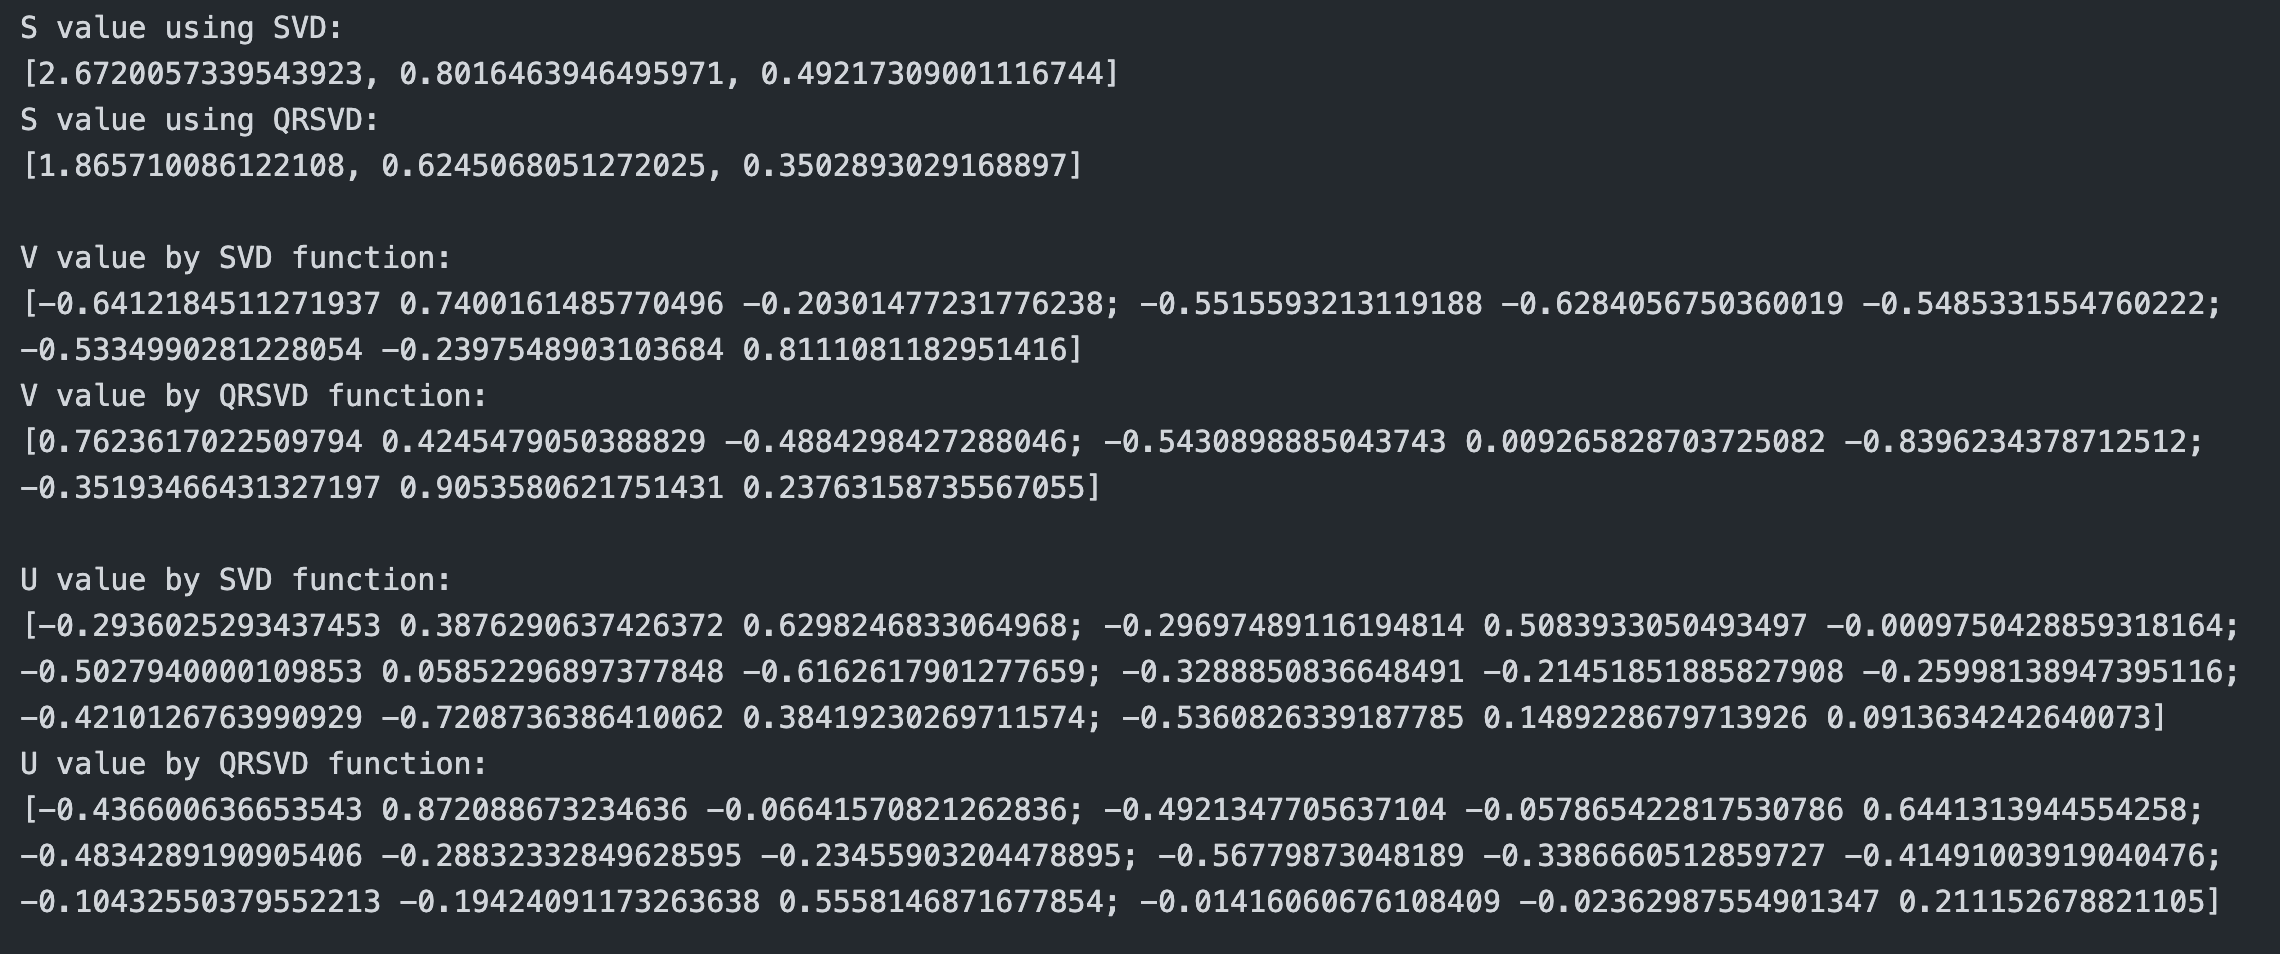
\includegraphics[scale=0.3]{SVD_QRSVD.png}
        \caption{Comparison of SVD values and QRSVD values}
        \label{fig:svd}
    \end{figure}
    \item This can solved as follows:
    \begin{align*}
     Q_1(R_1R_0) = (Q_1R_1)R_0 =  R_0^T R_0 [\because\ It\ is\ given\ that\ R_k^T=Q_{k+1}R_{k+1}]
    \end{align*}
    Now, $Q_1$ is orthonormal and both $R_1,R_0$ are upper triangular matrices. Thus, $Q_1(R_1R_0)$ is the QR decomposition of $R_0^TR_0$.
    \item part 1 can be shown as follows:
    \begin{align*}
        (R_1R_0)Q_1 & = R_1((Q_1R_1)^T)Q_1\\
        &= R_1 R_1^T Q_1^T Q_1
        &= R_1 R_1^T\ [\because Q_1\ is\ orthonormal]
    \end{align*}
    part 2 can be shown as follows:
    \begin{align*}
        R_1 R_1^T & = (Q_2R_2)^T(Q_2R_2)\\
        &= R_2^TQ_2^TQ_2R_2\\
        &= R_2^T R_2\ [\because Q_2\ is\ orthonormal]
    \end{align*}
    part 3 $B_0 = R_0^TR_0 = Q_1R_1R_0 = Q_1(R_1R_0)$\\
    part 3 $B_1 = R_2^TR_2 = R_1R_1^T = (R_1R_0)Q_1$\\
    Now, we know that $eigen(XY)=eigen(YX)$, thus \\
    $eig(B_0) = eig(Q_1(R_1R_0)) = eig((R_1R_0)Q_1) = eig(B_1)$.
    \item Considering the relation between $B_k$ and $B_{k+1}$ as follows:
    \begin{align*}
        B_k & = R_{2k}^TR_{2k}\\
         &= Q_{2k+1}R_{2k+1}R_{2k+1}^TQ_{2k+1}^T\\
         &= Q_{2k+1}(R^T_{2k+2}Q^T_{2k+2})(Q_{2k+2}R_{2k+2})Q^T_{2k+1}\\
         &= Q_{2k+1}B_{k+1}Q^T_{2k+1}\
    \end{align*}
    Now, for $B_0 = Q_1B_1Q_1^T =Q_1Q_3B_2Q_3^TQ_1^T =\ldots=Q_1Q_3\ldots Q_{2k-1}B_{K+1}Q^T_{2k-1}\ldots Q^T_3Q_1^T$.
    For each $B_i$ if we solve them one by one, we can see that it is actually the QR iteration of the general matrix as mentioned above. Hence, $B_k = R_{2k}^TR_{2k}$ are the QR iterations that are applied on the matrix $B_0 = R_{0}^TR_{0}$.
\end{enumerate}
\end{document}
